\section{Sentence Generation as Planning}
\label{sec:crisp}
In this section we review the original non-statistical {\sc crisp} system \cite{kollerstone2007}. 
Following {\sc spud} \cite{stonedoran1997}, {\sc crisp} is based on a declarative description of the sentence generation problem using {\sc tag}. Given a knowledge base, a communicative goal and a grammar, we require to find a grammatical {\sc tag} derivation that is consistent with this knowledge base and satisfies a communicative goal. A number of semantic and pragmatic constraints that must be satisfied by the solution can be added, for instance to enforce generation of unambiguous refering expressions. \newcite{kollerstone2007} describe how to encode this problem into an AI planning problem, that can be solved efficiently by off-the-shelf planners. We describe the general mechanism in the following section and then review the encoding into planning in section \ref{ssec:crispdomain}. 
\begin{figure*}[th]
\begin{center}
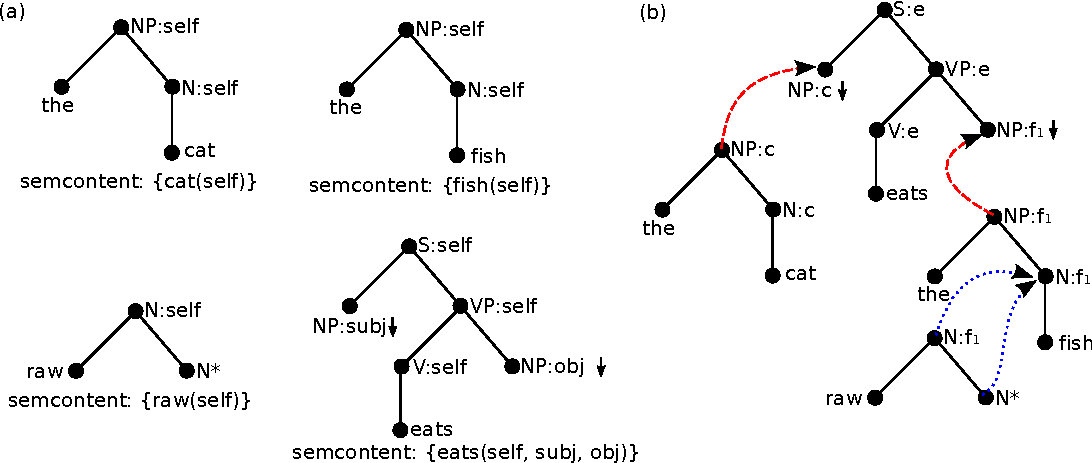
\includegraphics[width=.8\textwidth]{figures/grammar.pdf}
\caption{\label{fig:grammar}(a) An example grammar with semantic content. (b) A derivation for ``the cat eats the raw fish''. }
\end{center}
\end{figure*}

\subsection{Sentence Generation in CRISP}
Like {\sc spud}, {\sc crisp} uses an {\sc ltag} in which elementary trees are assigned semantic content. Each node in a {\sc crisp} elementary tree is associated with a semantic role. Semantic content is expressed as a set of literals, encoding relations between these roles. All nodes that dominate the lexical anchor are assigned the role `self', which intuitively corresponds to the event or individual described by this tree. Figure \ref{fig:grammar}(a) shows an example grammar of this type. 

In a derivation we may only include elementary trees whose semantic content has an instantiation in the knowledge base. For each substitution and adjunction, the semantic role associated with the role of the target node is unified with the `self' role of the child tree. For example, given the knowledge base 
{\it \{cat($i_2$), fish($i_3$), raw($i_3$), fish($i_4$), eats($i_1$,$i_2$,$i_3$)\}} and the grammar in \ref{fig:grammar}(a), {\sc crisp} could produce the derivation in \ref{fig:grammar}(b). Notice that {\sc crisp} can generate the unambiguos refering expression `the raw fish' for $i_3$, to distinguish it from $i_4$. For details on  refering expression generation in {\sc crisp} see \newcite{garoufikoller2010}.


\subsection{CRISP Planning Domains} 
\label{ssec:crispdomain}
Before we describe {\sc crisp}'s encoding of sentence generation as planning, we briefly review AI planning in general. 
A planning state is a conjunction of first order literals describing relations between some individuals. A planning problem consist of an initial state, a set of goal states and a set of planning operators that describe possible state transitions.  A solution to the problem is any sequence of actions (instantiated operators) that leads from the initial state to one of the goal states. Planning problems can be solved efficiently by general purpose planning systems such as 
{\sc ff} \cite{hoffmannnebel2001}.  
% Planning problems can be written in a standard notation ({\sc pddl}\footnote{Planning Domain Description Language}, \newcite{gerevinietal2009}).
     
In {\sc crisp} planning states correspond to partial {\sc tag} derivations and record open substitution and adjunction sites, semantic individuals associated with them, and parts of the communicative goal that have not yet been expressed.  The initial state also encodes the knowledge base and the communicative goal. Each planning operator contributes a new elementary tree to the derivation and at the same time satisfies part of the communicative goal, as described in the previous section. In a goal state there are no open substitution sites left and all literals in the communicative goal have been expressed. 
\begin{figure}[t]
\begin{center}
\planaction{\bf subst-t28-eats-S(u,~x1,~x2,~x3)}{referent(u,~x1),\\ subst(S,~u), eats(x1,~x2,~x3)}{
$\lnot$needtoexpr(pred-eats,~x1,~x2,~x3),\\ $\lnot$subst(S,~u),\\
subst(NP,~subj), subst(NP,~obj),\\ referent(subj,~x2), referent(obj,~x3)\\
adj(VP, u), adj(V, u), adj(S, u)}\\\smallskip

\planaction{\bf subst-t3-cat-NP(u,~x1)}{referent(u,~x1),\\ subst(NP,~u), cat(x1)}{
$\lnot$needtoexpr(pred-cat,~x1),\\ $\lnot$subst(NP,~u),\\
adj(N, u), adj(NP, u)}\\ \smallskip


\planaction{\bf subst-t5-raw-N(u,~x1)}{referent(u,~x1),\\ adj(N,~u), raw(x1)}{
$\lnot$needtoexpr(pred-raw,~x1),\\ $\lnot$adj(N,~u)}\\\smallskip
\end{center}
\caption{\label{fig:crisp-operators} {\sc crisp} operators for some of the elementary trees in figure \ref{fig:grammar}.}
\end{figure}


Figure \ref{fig:crisp-operators} shows planning operators for part of the grammar in figure \ref{fig:grammar}(a).
The preconditions of the operators require that a suitable open substitution node (i.e. of the correct category) or internal node for adjunction exists in the partial derivation. In the operator effect, open substitution nodes are closed and new identifiers are created for each substitution node and internal node in the new tree. Given the knowlede base from above, a plan corresponding to the derivation in figure \ref{fig:grammar} would be $\langle${\it S-eats-1(root, i1, i2, i3), NP-cat-2(subj-1, i2), NP-fish-3(obj-1, i3), N-raw-4(obj-1, i3)}$\rangle$

\subsection{CRISP and Large Grammars}
Using {\sc crisp} with large, treebank induced grammars can lead to overgeneration, 
%Such trees contain many internal nodes that are open for adjunction but will not necessarily be filled in a derivation for a given input communicative goal. Attaching to the wrong node can produce invalid or disprefered word order. 
due to the high lexical ambiguity of possible, structurally different trees (supertags) for a given word. We illustrate this problem in figure \ref{fig:overgen}. Assuming a grammar that includes trees for both right adjoining ($t13$) and left adjoining PPs ($t252$), both derivations (a) and (b) are {\it grammatical} derivations that satisfy the same communicative goal. However, most readers disprefer the reading in (b). 
Clearly, to use {\sc crisp} with such a grammar we need a method of distinguishing good derivations from bad ones. In section \ref{sec:experiments} we provide empirical evidence for this problem and show how it is solved by the approach we describe in the next section. 
\begin{figure}
\begin{center}
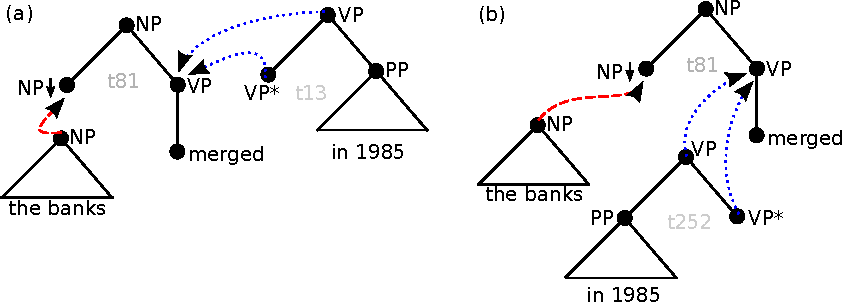
\includegraphics[width=.3\textwidth]{figures/overgen.pdf}
\caption{\label{fig:overgen} Two derivations with a large grammar, that satisfy the same communicative goal. Sentence (b) is disprefered by most readers.}
\end{center}
\end{figure} 

